\documentclass[10pt,a4paper]{report}
%\usepackage[latin1]{inputenc}
\usepackage{blindtext}
\usepackage{multicol}
\usepackage[utf8]{inputenc}
\usepackage{amsmath}
\makeatletter
\newcommand\xleftrightarrow[2][]{%
  \ext@arrow 9999{\longleftrightarrowfill@}{#1}{#2}}
\newcommand\longleftrightarrowfill@{%
  \arrowfill@\leftarrow\relbar\rightarrow}
\makeatother
\usepackage{amsfonts}
\usepackage{amssymb}
\usepackage{graphicx}
\usepackage{multicol}
\usepackage{tabularx}
\usepackage{tikz}
\usepackage{hyperref}
\hypersetup{
colorlinks=true,
linkcolor=blue,
filecolor=blue,
citecolor = black,
urlcolor=blue,
}
\usetikzlibrary{arrows,shapes,automata,petri,positioning,calc}
\usepackage{hyperref}
\usepackage{tikz}
\usetikzlibrary{matrix,calc}
\newcommand{\myvec}[1]{\ensuremath{\begin{pmatrix}#1\end{pmatrix}}}
\usepackage[margin=0.5in]{geometry}
\providecommand{\norm}[1]{\left\lVert#1\right\rVert}
\providecommand{\brak}[1]{\ensuremath{\left(#1\right)}}
\providecommand{\lbrak}[1]{\ensuremath{\left(#1\right.}}
\providecommand{\rbrak}[1]{\ensuremath{\left.#1\right)}}
\providecommand{\sbrak}[1]{\ensuremath{{}\left[#1\right]}}
%\newcommand{\myvec}[1]{\ensuremath{\begin{pmatrix}#1\end{pmatrix}}}
\let\vec\mathbf
\newcommand{\mydet}[1]{\ensuremath{\begin{vmatrix}#1\end{vmatrix}}}
%\newcommand{\myvec}[1]{\ensuremath{\begin{pmatrix}#1\end{pmatrix}}}
%\let\vec\mathbf
\providecommand{\mtx}[1]{\mathbf{#1}}
\newenvironment{Figure}
  {\par\medskip\noindent\minipage{\linewidth}}
  {\endminipage\par\medskip}
\begin{document}
%--------------------logo figure-------------------------%
\begin{figure*}[!tbp]
  \centering
  \begin{minipage}[b]{0.4\textwidth}
   
\includegraphics[scale=0.5]{iithlogo.png} 
  \end{minipage}
  \hfill
  \vspace{5mm}\begin{minipage}[b]{0.4\textwidth}
\raggedleft 
\includegraphics[scale=0.5]{nrc.jpeg} 
  \end{minipage}\vspace{0.2cm}
\end{figure*}
%--------------------name & rollno-----------------------
\raggedright 
\begin{center}
\Large \textbf{Conics Assignment}\hspace{2.5cm} %
\end{center}
\begin{center}
\hspace{0.5cm}
\textbf{Name}:\hspace{2mm}Rupa Sai Sreshta Vallabhaneni\hspace{1cm}
\date{25-September-2022}
\end{center}
%\begin{center}
%\end{center}  
%\normalsize \textbf{Roll No.} :\hspace{1mm} FWC22047\vspace{1cm}
%\begin{multicols}{2}
%\begin{tableofcontents}
%\begin{tableofcontents}
\begin{multicols}{2}
\section*{Problem Statement:}
Consider a branch of hyperbola $x^{2}-2y^{2}-2\sqrt{2}x-4\sqrt{2}y-6=0$ with vertex at the point $\vec{A}$. Let $\vec{B}$ be one of the end point of its latus rectum. If $\vec{C}$ is the focus of the hyperbola nearest to the point $\vec{A}$, then the area of triangle $\vec{A}\vec{B}\vec{C}$ is?
\section*{Construction:}
\hspace{0.25cm}
\begin{tabular}{|c|c|c|}
	\hline
	\textbf{Symbol}&\textbf{Value}&\textbf{Description}\\
	\hline
	$\vec{C}$&$\myvec{\sqrt{2} \\ -\sqrt{2}}$&Center of hyperbola\\
	\hline
\end{tabular}
%\hspace{2cm}\\
\vspace{0.5cm}\\
%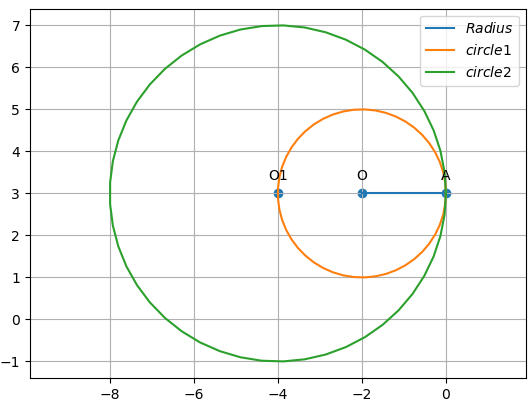
\includegraphics[scale=0.4]{circle2.png}
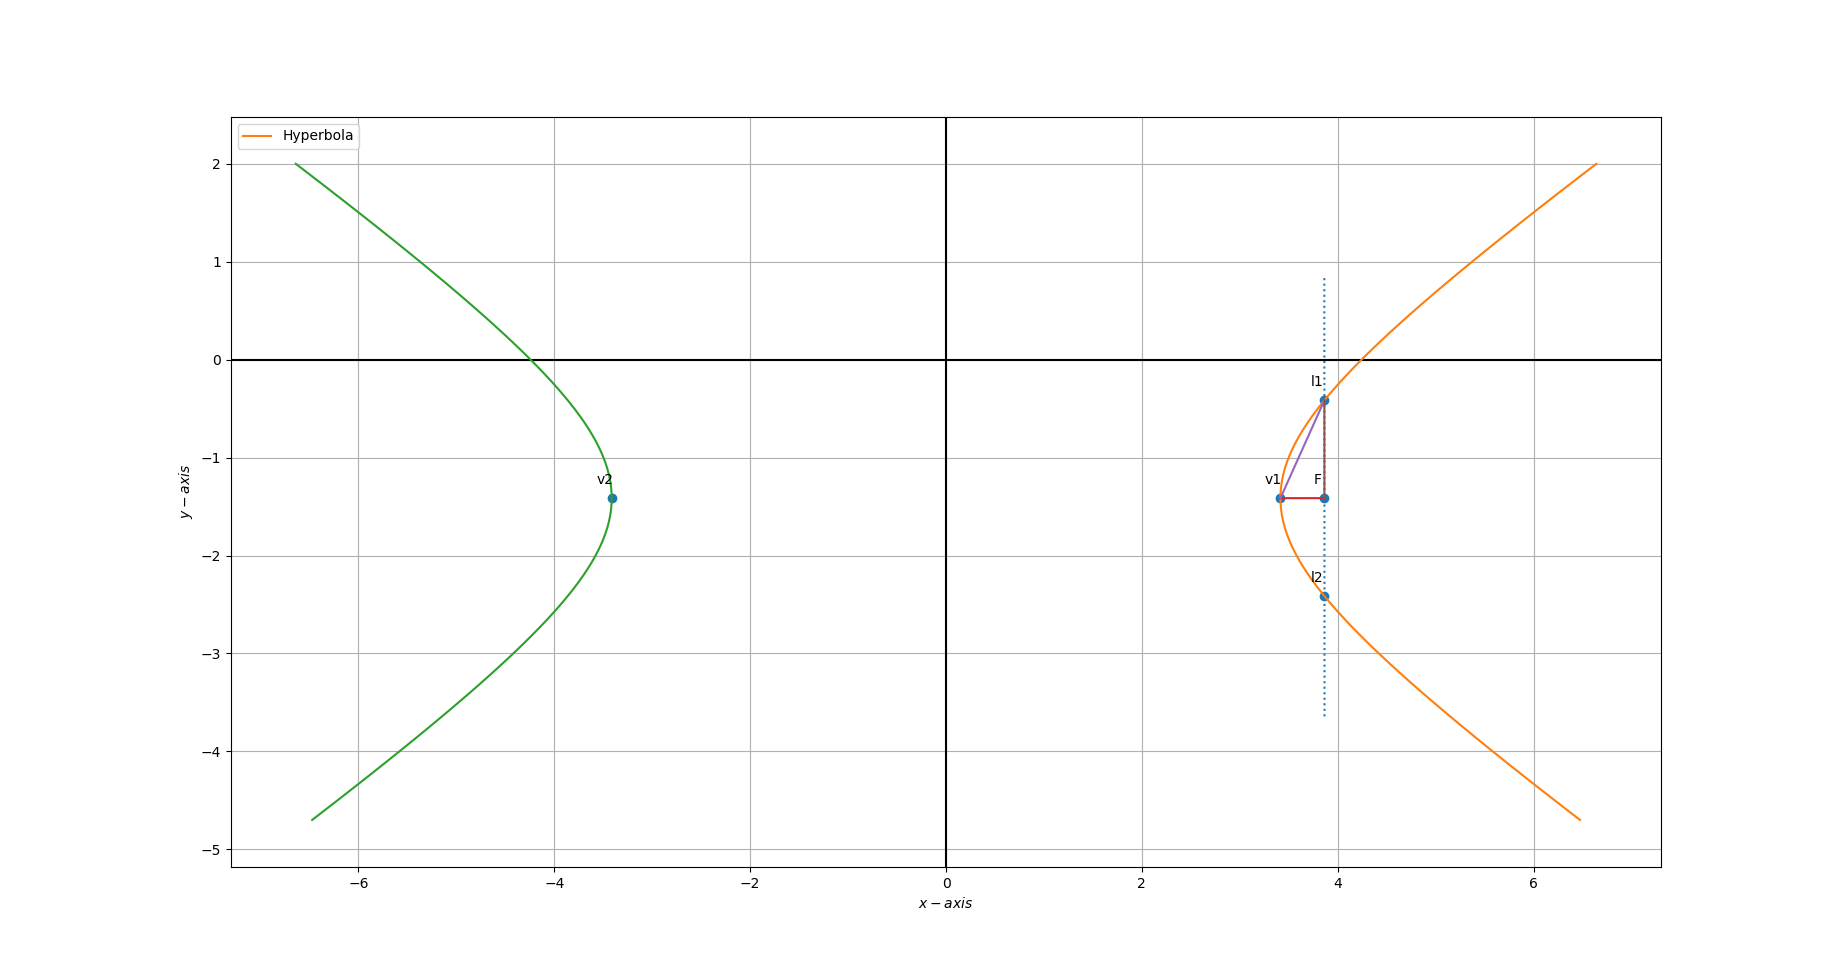
\includegraphics[scale=0.21]{hypfig.png}
\begin{center}
Figure of construction
\end{center} 
You can download the python code for generating above hyperbola from the below link
\vspace{0.25cm}\\
\boxed{Github link: \href{https://github.com/RupaSaiSreshta/FWC}{https://github.com/RupaSaiSreshta/FWC}}

\section*{Solution:}
The given Hyperbola equation is 
\vspace{0.25cm}
\begin{align}
\vec{x}^{\top}\vec{V}\vec{x}+2\vec{u}^{\top}\vec{x}+f=0
\end{align}
%\vspace{0.25cm}\\
\begin{align}
\vec{V}=\vec{ \begin{pmatrix}1 & 0 \\ 0 & -2 \end{pmatrix}}, 
\end{align}
\begin{align}
\vec{u}=\vec{ \begin{pmatrix}-\sqrt{2} \\ -2\sqrt{2} \end{pmatrix}},
\end{align}
\begin{align}
f = -6.
\end{align}
Eigen values of $\vec{V}$ are $\lambda_1$ and $\lambda_2$
\vspace{0.25cm}\\
Here $\lambda_1$ = -2  , $\lambda_2$ = 1
\vspace{0.25cm}\\
Now eccentricity of hyperbola is 
\vspace{0.25cm}\\
\begin{equation}
e=\sqrt{1-\frac{\lambda_1}{\lambda_2}}
\end{equation}
\vspace{0.25cm}\\
Center of the hyperbola
\begin{align}
\vec{C}=-\vec{V}^{-1}\vec{u}
\end{align}
By solving we get
\begin{align} 
\vec{C} &= \myvec{\sqrt{2} \\ -\sqrt{2}} 
\end{align}
\textbf{For vertex:}
\vspace{0.25cm}\\
Take the major axis equation 
\begin{equation}
c=-\sqrt{2}
\end{equation}
\vspace{0.25cm}\\
Now, Take the formula for line intersecting to the conic 
\vspace{0.25cm}\\
\begin{equation}
\vec{x}=\vec{q}+\mu_i\vec{m}
\end{equation}
%\vspace{0.25cm}\\
\begin{align} 
\vec{q} &= \myvec{\sqrt{2} \\ -\sqrt{2}} 
\end{align}
\begin{align} 
\vec{m} &= \myvec{1 \\ 0} 
\end{align}
\begin{multline}
\mu_i = \frac{1}
{
\vec{m}^T\vec{V}\vec{m}
}
\lbrak{-\vec{m}^T\brak{\vec{V}\vec{q}+\vec{u}}}
\\
\pm
\rbrak{\sqrt{
\sbrak{
\vec{m}^T\brak{\vec{V}\vec{q}+\vec{u}}
}^2
-
\brak
{
\vec{q}^T\vec{V}\vec{q} + 2\vec{u}^T\vec{q} +f
}
\brak{\vec{m}^T\vec{V}\vec{m}}
}
}
\end{multline}
By solving we get 
%\vspace{0.25cm}\\
\begin{align}
\mu_i=\pm 2
\end{align}

%\vspace{0.25cm}\\
Now substitute in eq 6 and adding center 
\vspace{0.25cm}\\
we get
\vspace{0.25cm}\\
\begin{equation}
\vec{V_1} = \myvec{2+\sqrt{2} \\ -\sqrt{2}}
\end{equation}
\begin{equation}
\vec{V_2} = \myvec{-2+\sqrt{2} \\ -\sqrt{2}}
\end{equation}
\vspace{0.25cm}\\
\textbf{For Focus:}
\vspace{0.25cm}\\
\begin{equation}
\vec{F} = \pm e \sqrt{\frac{|f_0|}{\lambda_2(1-e^2)}} \vec{e_1}
\end{equation}
\vspace{0.25cm}\\
By solving and adding center we get 
\vspace{0.25cm}\\
\begin{equation}
\vec{F_1} = \myvec{\sqrt{6}+\sqrt{2} \\ -\sqrt{2}}
\end{equation}
\begin{equation}
\vec{F_2} = \myvec{-\sqrt{6}+\sqrt{2} \\ -\sqrt{2}}
\end{equation}
\vspace{0.25cm}\\
\textbf{For Latus rectum:}
\vspace{0.25cm}\\
Draw the tangent to vertex $\vec{V_1}$ and find the direction vector of tangent.
\vspace{0.25cm}\\
Then draw the line parallel to tangent  $\vec{V_1}$ through the focus point
\vspace{0.25cm}\\
Now, Take the formula for line intersecting to the conic 
\vspace{0.25cm}\\
\begin{equation}
\vec{x}=\vec{q}+\mu_i\vec{m}
\end{equation}
\begin{align} 
\vec{q} &=  \myvec{\sqrt{6}+\sqrt{2} \\ -\sqrt{2}}
\end{align}
\begin{align} 
\vec{m} &= \myvec{0 \\ 1} 
\end{align}

\begin{multline}
\mu_i = \frac{1}
{
\vec{m}^T\vec{V}\vec{m}
}
\lbrak{-\vec{m}^T\brak{\vec{V}\vec{q}+\vec{u}}}
\\
\pm
\rbrak{\sqrt{
\sbrak{
\vec{m}^T\brak{\vec{V}\vec{q}+\vec{u}}
}^2
-
\brak
{
\vec{q}^T\vec{V}\vec{q} + 2\vec{u}^T\vec{q} +f
}
\brak{\vec{m}^T\vec{V}\vec{m}}
}
}
\end{multline}
By solving we get 
%\vspace{0.25cm}\\
\begin{align}
\mu_i=\pm 1
\end{align}
%\vspace{0.25cm}\\
Now substitute in eq 15 and adding center 
\vspace{0.25cm}\\
we get
\vspace{0.25cm}\\
\begin{equation}
\vec{L_1} = \myvec{\sqrt{6}+\sqrt{2} \\ 1-\sqrt{2}}
\end{equation}
\begin{equation}
\vec{L_2} = \myvec{\sqrt{6}+\sqrt{2} \\ -1-\sqrt{2}}
\end{equation}
\textbf{For Area of triangle:}
\vspace{0.25cm}\\
For finding area of triangle $\vec{V_1}\vec{L_1}\vec{F_1}$
\begin{equation}
\vec{Ar}=\frac{1}{2}\norm{(\vec{(V_1-L_1)}\times\vec{(F_1-L_1)})}
\end{equation}
\begin{equation}
\vec{V_1} = \myvec{2+\sqrt{2} \\ -\sqrt{2}}
\end{equation}
\begin{equation}
\vec{L_1} = \myvec{\sqrt{6}+\sqrt{2} \\ 1-\sqrt{2}}
\end{equation}
\begin{equation}
\vec{F_1} = \myvec{\sqrt{6}+\sqrt{2} \\ -\sqrt{2}}
\end{equation}
\vspace{0.25cm}\\
Substitute these values in eq 21
\vspace{0.25cm}\\
By solving we get
\begin{equation}
 \boxed { \vec{Ar} = \sqrt{\frac{3}{2}} - 1}
\end{equation}
\end{multicols}
\end{document}
